\documentclass{article}\usepackage[]{graphicx}\usepackage[]{color}
%% maxwidth is the original width if it is less than linewidth
%% otherwise use linewidth (to make sure the graphics do not exceed the margin)
\makeatletter
\def\maxwidth{ %
  \ifdim\Gin@nat@width>\linewidth
    \linewidth
  \else
    \Gin@nat@width
  \fi
}
\makeatother

\definecolor{fgcolor}{rgb}{0.345, 0.345, 0.345}
\newcommand{\hlnum}[1]{\textcolor[rgb]{0.686,0.059,0.569}{#1}}%
\newcommand{\hlstr}[1]{\textcolor[rgb]{0.192,0.494,0.8}{#1}}%
\newcommand{\hlcom}[1]{\textcolor[rgb]{0.678,0.584,0.686}{\textit{#1}}}%
\newcommand{\hlopt}[1]{\textcolor[rgb]{0,0,0}{#1}}%
\newcommand{\hlstd}[1]{\textcolor[rgb]{0.345,0.345,0.345}{#1}}%
\newcommand{\hlkwa}[1]{\textcolor[rgb]{0.161,0.373,0.58}{\textbf{#1}}}%
\newcommand{\hlkwb}[1]{\textcolor[rgb]{0.69,0.353,0.396}{#1}}%
\newcommand{\hlkwc}[1]{\textcolor[rgb]{0.333,0.667,0.333}{#1}}%
\newcommand{\hlkwd}[1]{\textcolor[rgb]{0.737,0.353,0.396}{\textbf{#1}}}%

\usepackage{framed}
\makeatletter
\newenvironment{kframe}{%
 \def\at@end@of@kframe{}%
 \ifinner\ifhmode%
  \def\at@end@of@kframe{\end{minipage}}%
  \begin{minipage}{\columnwidth}%
 \fi\fi%
 \def\FrameCommand##1{\hskip\@totalleftmargin \hskip-\fboxsep
 \colorbox{shadecolor}{##1}\hskip-\fboxsep
     % There is no \\@totalrightmargin, so:
     \hskip-\linewidth \hskip-\@totalleftmargin \hskip\columnwidth}%
 \MakeFramed {\advance\hsize-\width
   \@totalleftmargin\z@ \linewidth\hsize
   \@setminipage}}%
 {\par\unskip\endMakeFramed%
 \at@end@of@kframe}
\makeatother

\definecolor{shadecolor}{rgb}{.97, .97, .97}
\definecolor{messagecolor}{rgb}{0, 0, 0}
\definecolor{warningcolor}{rgb}{1, 0, 1}
\definecolor{errorcolor}{rgb}{1, 0, 0}
\newenvironment{knitrout}{}{} % an empty environment to be redefined in TeX

\usepackage{alltt}
\usepackage{fullpage}

\title{STAT 675, HW \#5}
\author{Dominic D LaRoche}
\IfFileExists{upquote.sty}{\usepackage{upquote}}{}
\begin{document}

\begin{itemize}
\item{10.1} Histogram estimate of the density of a standard lognormal using Sturge's rule and Doane's correction for skewness.\\

Using code adapted from the book example 10.1.\\

\begin{kframe}
\begin{alltt}
\hlkwd{require}(xtable)
\end{alltt}


{\ttfamily\noindent\itshape\color{messagecolor}{\#\# Loading required package: xtable}}\begin{alltt}
\hlkwd{set.seed}(3)
n <- 100
x <- \hlkwd{rlnorm}(n)
\hlcom{# calc breaks according to Sturges' Rule}
nclass <- \hlkwd{ceiling}(1 + \hlkwd{log2}(n))
cwidth <- \hlkwd{diff}(\hlkwd{range}(x)/nclass)
breaks <- \hlkwd{min}(x) + cwidth * 0:nclass

h.sturges <- \hlkwd{hist}(x, breaks = breaks, freq = FALSE, main = \hlstr{"hist: Sturges"})
\end{alltt}
\end{kframe}
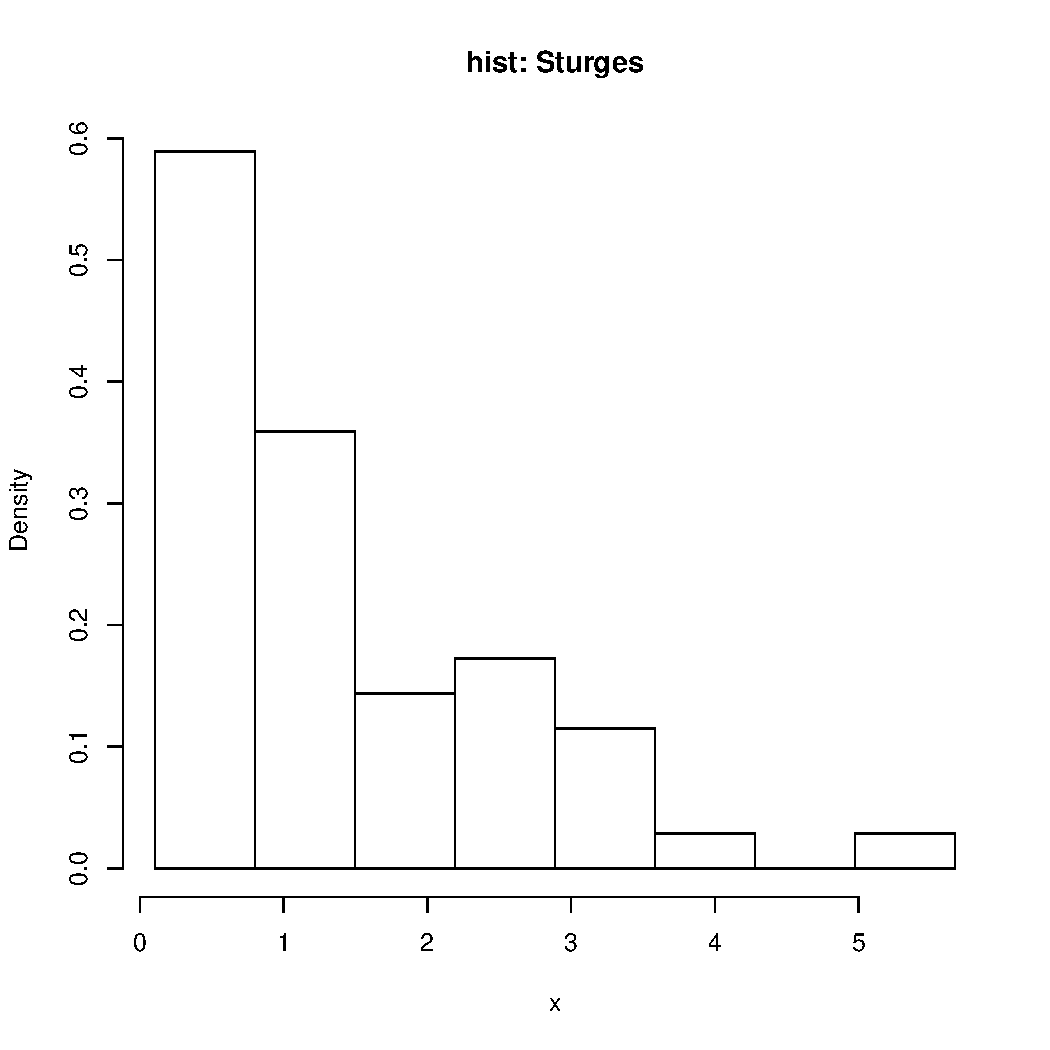
\includegraphics[width=\maxwidth]{figure/ten11} 
\begin{kframe}\begin{alltt}

\hlcom{# apply correction for skewness}
\hlkwd{require}(moments)
\end{alltt}


{\ttfamily\noindent\itshape\color{messagecolor}{\#\# Loading required package: moments}}\begin{alltt}
sk <- \hlkwd{skewness}(x)
sesk <- \hlkwd{sqrt}((6 * (n - 2))/((n + 1) * (n + 3)))
k <- \hlkwd{log2}(1 + sk/sesk)
nclass.d <- \hlkwd{ceiling}(1 + \hlkwd{log2}(n) + k)
cwidth.d <- \hlkwd{diff}(\hlkwd{range}(x)/nclass.d)
breaks.d <- \hlkwd{min}(x) + cwidth.d * 0:nclass.d
h.doane <- \hlkwd{hist}(x, breaks = breaks.d, freq = FALSE, main = \hlstr{"hist: Doane"})
\end{alltt}
\end{kframe}
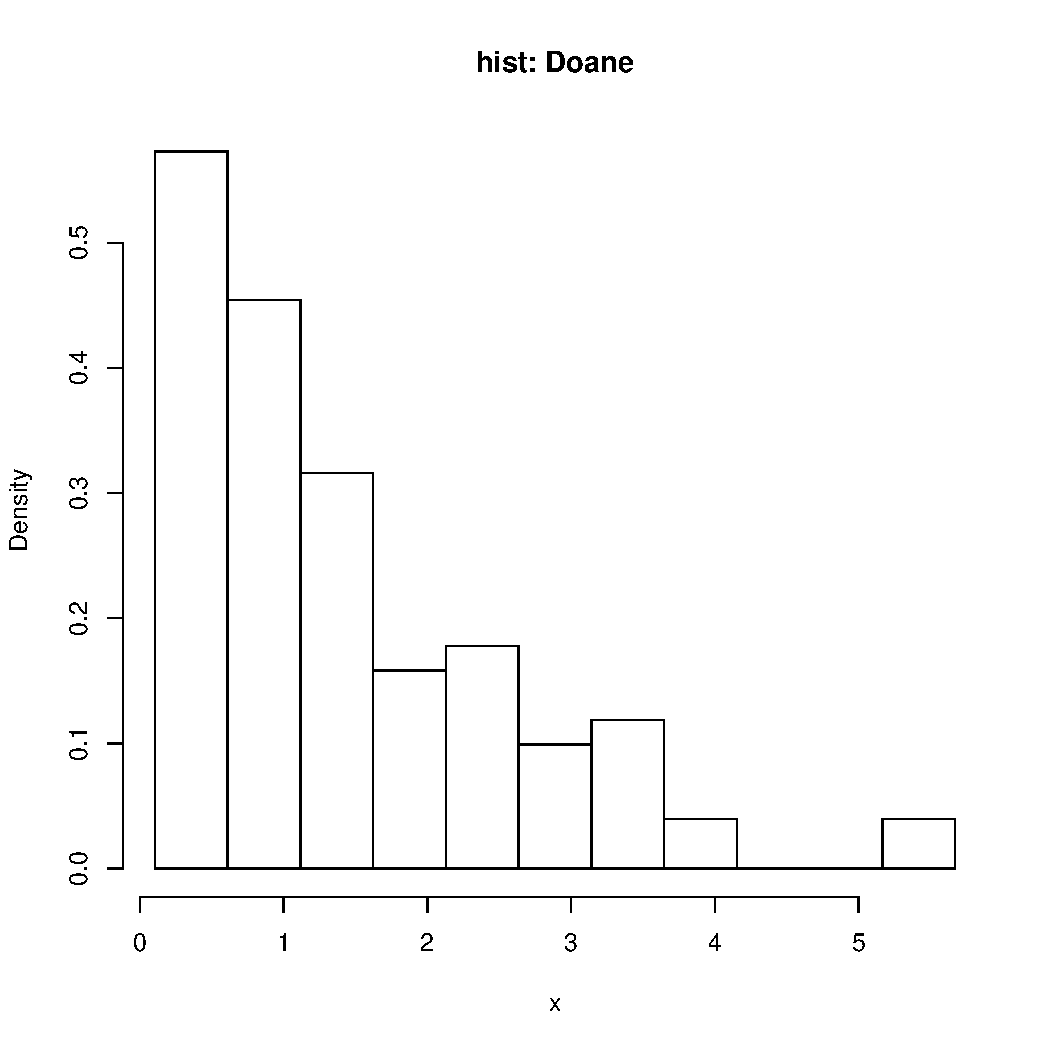
\includegraphics[width=\maxwidth]{figure/ten12} 
\begin{kframe}\begin{alltt}

\hlcom{# compare density to the theoretical values}
lnorm.dens <- \hlkwd{dlnorm}(\hlkwd{qlnorm}(\hlkwd{seq}(0.1, 0.9, 0.1)))
compare.doane <- \hlkwd{rbind}(h.doane$breaks[\hlkwd{which}(h.doane$breaks <= \hlkwd{max}(\hlkwd{qlnorm}(\hlkwd{seq}(0.1, 
    0.9, 0.1))))], h.doane$density[\hlkwd{which}(h.doane$breaks <= \hlkwd{max}(\hlkwd{qlnorm}(\hlkwd{seq}(0.1, 
    0.9, 0.1))))], \hlkwd{dlnorm}(h.doane$breaks[\hlkwd{which}(h.doane$breaks <= \hlkwd{max}(\hlkwd{qlnorm}(\hlkwd{seq}(0.1, 
    0.9, 0.1))))]))
compare.sturges <- \hlkwd{rbind}(h.sturges$breaks[\hlkwd{which}(h.sturges$breaks <= \hlkwd{max}(\hlkwd{qlnorm}(\hlkwd{seq}(0.1, 
    0.9, 0.1))))], h.sturges$density[\hlkwd{which}(h.sturges$breaks <= \hlkwd{max}(\hlkwd{qlnorm}(\hlkwd{seq}(0.1, 
    0.9, 0.1))))], \hlkwd{dlnorm}(h.sturges$breaks[\hlkwd{which}(h.sturges$breaks <= \hlkwd{max}(\hlkwd{qlnorm}(\hlkwd{seq}(0.1, 
    0.9, 0.1))))]))
\hlkwd{rownames}(compare.doane) <- \hlkwd{rownames}(compare.sturges) <- \hlkwd{c}(\hlstr{"Breaks within the first 90\textbackslash{}\textbackslash{}% of the theoretical density"}, 
    \hlstr{"Estimates Density"}, \hlstr{"Theoretical Density"})
\hlkwd{xtable}(compare.sturges, caption = \hlstr{"Comparison of the Sturges density estimate with theoretical values"})
\end{alltt}
\end{kframe}% latex table generated in R 2.15.3 by xtable 1.7-1 package
% Sun Apr 20 13:54:28 2014
\begin{table}[ht]
\centering
\begin{tabular}{rrrrrrr}
  \hline
 & 1 & 2 & 3 & 4 & 5 & 6 \\ 
  \hline
Breaks within the first 90$\backslash$\% of the theoretical density & 0.10 & 0.80 & 1.50 & 2.19 & 2.89 & 3.58 \\ 
  Estimates Density & 0.59 & 0.36 & 0.14 & 0.17 & 0.11 & 0.03 \\ 
  Theoretical Density & 0.30 & 0.49 & 0.25 & 0.13 & 0.08 & 0.05 \\ 
   \hline
\end{tabular}
\caption{Comparison of the Sturges density estimate with theoretical values} 
\end{table}
\begin{kframe}\begin{alltt}
\hlkwd{xtable}(compare.doane, caption = \hlstr{"Comparison of the Doane corrected density estimates with the theoretical values"})
\end{alltt}
\end{kframe}% latex table generated in R 2.15.3 by xtable 1.7-1 package
% Sun Apr 20 13:54:28 2014
\begin{table}[ht]
\centering
\begin{tabular}{rrrrrrrr}
  \hline
 & 1 & 2 & 3 & 4 & 5 & 6 & 7 \\ 
  \hline
Breaks within the first 90$\backslash$\% of the theoretical density & 0.10 & 0.61 & 1.12 & 1.62 & 2.13 & 2.63 & 3.14 \\ 
  Estimates Density & 0.57 & 0.45 & 0.32 & 0.16 & 0.18 & 0.10 & 0.12 \\ 
  Theoretical Density & 0.30 & 0.58 & 0.36 & 0.22 & 0.14 & 0.09 & 0.07 \\ 
   \hline
\end{tabular}
\caption{Comparison of the Doane corrected density estimates with the theoretical values} 
\end{table}



The Doane correction adds 3 more bars (and breaks) than the Sturges histogram but only one of these was within the first 9 deciles.  In general both methods did a poor job of estimating the density near 0 but got better further from zero.  The Doane estimate did slightly better in genreral.\\

\item[10.6]  Normal reference rule ASH estimate of the eruptions density.\\

I will use the ash function since it seems well equiped for this sort of thing.\\
\begin{knitrout}
\definecolor{shadecolor}{rgb}{0.969, 0.969, 0.969}\color{fgcolor}\begin{kframe}
\begin{alltt}
\hlkwd{require}(MASS)
\end{alltt}


{\ttfamily\noindent\itshape\color{messagecolor}{\#\# Loading required package: MASS}}\begin{alltt}
\hlkwd{require}(ash)
\end{alltt}


{\ttfamily\noindent\itshape\color{messagecolor}{\#\# Loading required package: ash}}\begin{alltt}
erupt <- faithful$eruptions
n <- \hlkwd{length}(erupt)
\hlcom{# scott's normal reference rule}
h <- 2.576 * \hlkwd{sd}(erupt) * n^(-0.2)
R <- \hlkwd{diff}(\hlkwd{range}(erupt))
numbin <- \hlkwd{ceiling}(R * 20/h)
\hlcom{# set the interval by adding 20% of the range to either end of the}
\hlcom{# interval}
interval <- \hlkwd{c}(\hlkwd{range}(erupt)[1] - R * 0.2, \hlkwd{range}(erupt)[2] + R * 0.2)
bins <- \hlkwd{bin1}(erupt, nbin = numbin, ab = interval)
ashest <- \hlkwd{ash1}(bins = bins, m = 10, kopt = \hlkwd{c}(2, 2))
\hlkwd{plot}(ashest, type = \hlstr{"l"})
\end{alltt}
\end{kframe}
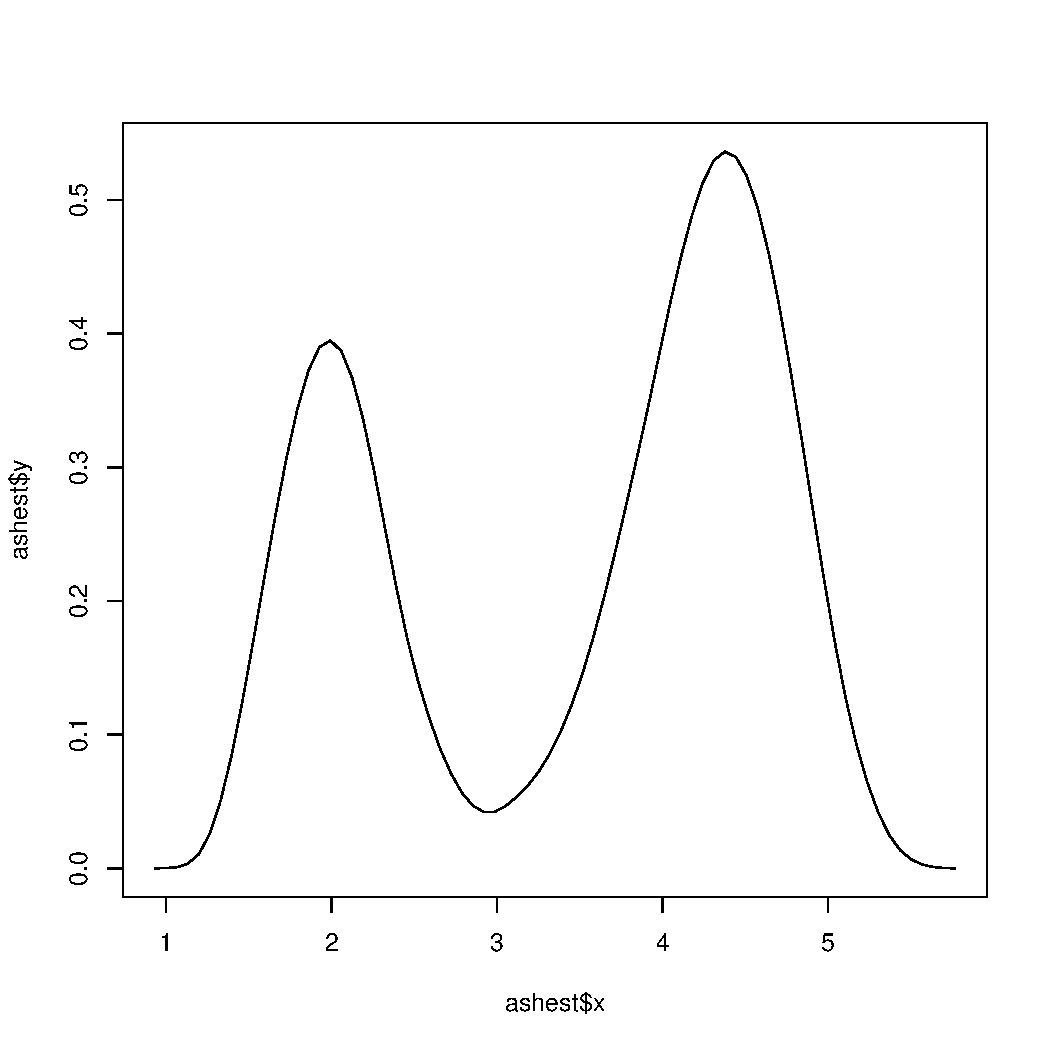
\includegraphics[width=\maxwidth]{figure/ten6} 

\end{knitrout}


\item[10.8]  Kernel density estimates of the buffalo data.\\

\begin{knitrout}
\definecolor{shadecolor}{rgb}{0.969, 0.969, 0.969}\color{fgcolor}\begin{kframe}
\begin{alltt}
\hlkwd{require}(gss)
\end{alltt}


{\ttfamily\noindent\itshape\color{messagecolor}{\#\# Loading required package: gss}}\begin{alltt}
\hlkwd{data}(buffalo)
bws <- \hlkwd{c}(\hlstr{"nrd0"}, \hlstr{"nrd"}, \hlstr{"ucv"}, \hlstr{"SJ"})
kerns <- \hlkwd{c}(\hlstr{"gaussian"}, \hlstr{"biweight"})
\hlkwd{for} (i in 1:\hlkwd{length}(kerns)) \{
    \hlkwd{par}(mfrow = \hlkwd{c}(2, 2))
    kern <- kerns[i]
    \hlkwd{for} (j in 1:\hlkwd{length}(bws)) \{
        \hlkwd{plot}(\hlkwd{density}(buffalo, bw = \hlkwd{paste0}(bws[j]), kernel = \hlkwd{paste0}(kern)), main = \hlkwd{paste0}(kern, 
            \hlstr{" with "}, bws[j]))
    \}
\hlcom{    # plot(truehist(buffalo))}
    \hlkwd{par}(mfrow = \hlkwd{c}(1, 1))
\}
\end{alltt}
\end{kframe}
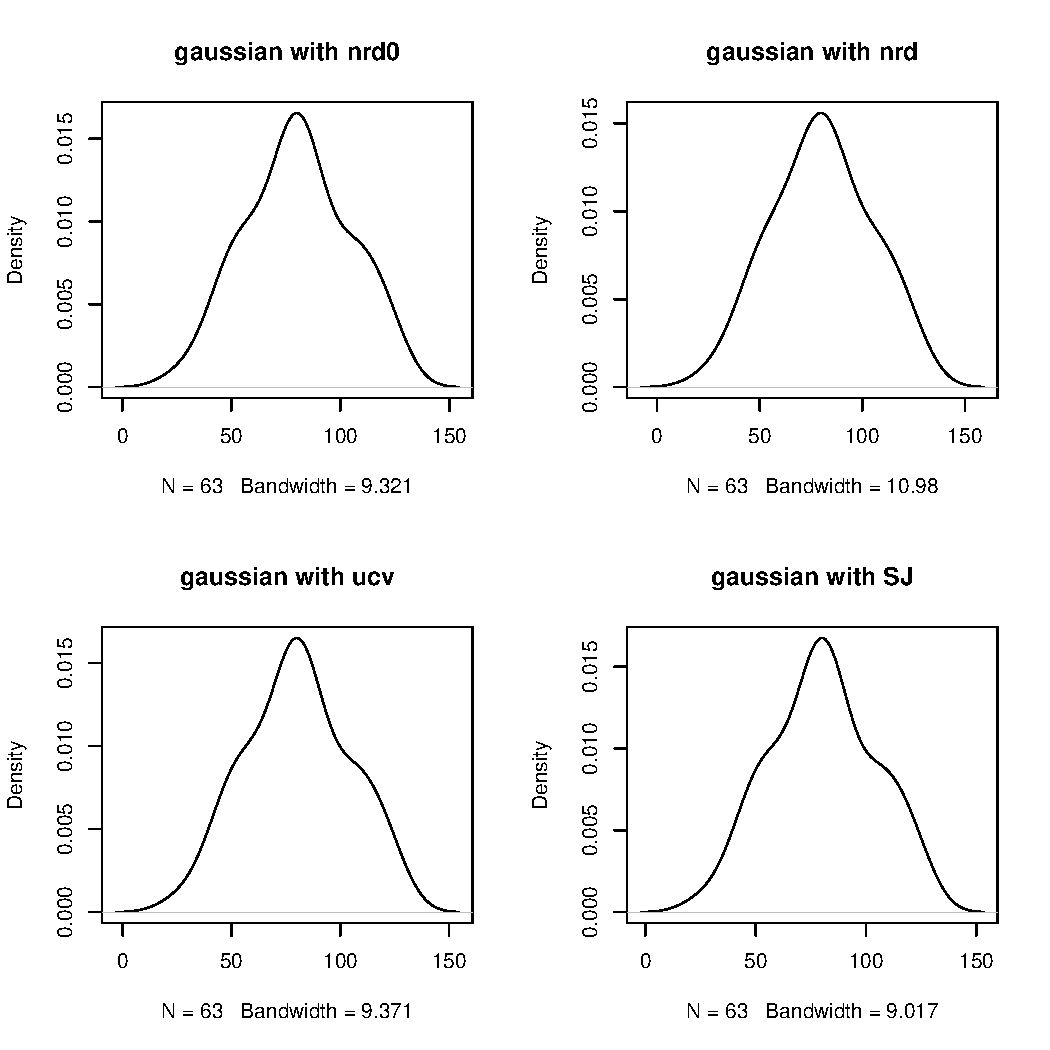
\includegraphics[width=\maxwidth]{figure/ten81} 

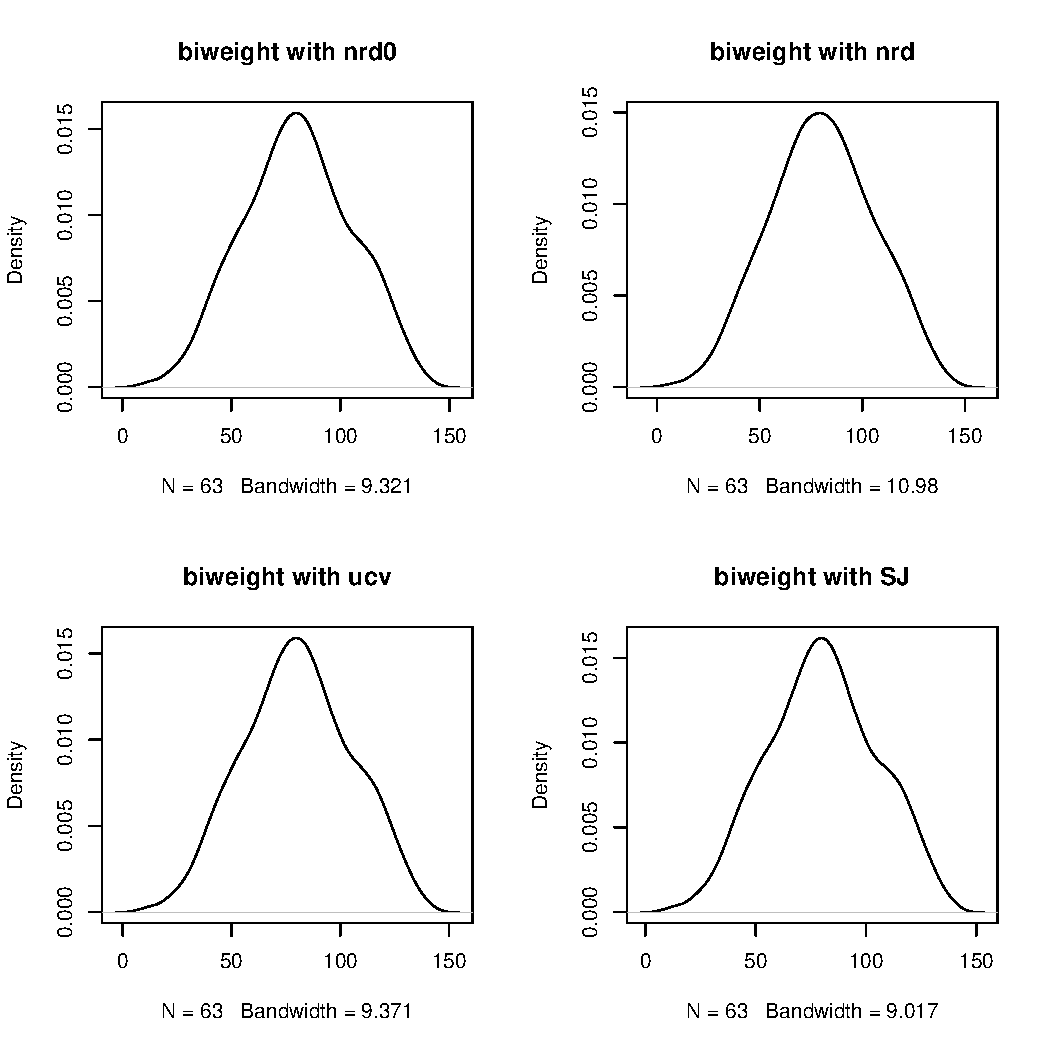
\includegraphics[width=\maxwidth]{figure/ten82} 

\end{knitrout}

It appears that the bandwidth choice has more of an impact than the kernel choice.\\

\item[10.9] KDE of a normal mixture.\\

\begin{knitrout}
\definecolor{shadecolor}{rgb}{0.969, 0.969, 0.969}\color{fgcolor}\begin{kframe}
\begin{alltt}
\hlkwd{set.seed}(3)
n <- 100
mu <- \hlkwd{sample}(\hlkwd{c}(0, 3), size = n, replace = T)
x <- \hlkwd{rnorm}(n, mu)
\hlkwd{par}(mfrow = \hlkwd{c}(2, 2))
\hlkwd{for} (i in 1:\hlkwd{length}(bws)) \{
    \hlkwd{plot}(\hlkwd{density}(x, bw = \hlkwd{paste0}(bws[i]), kernel = \hlstr{"gaussian"}), main = \hlkwd{paste0}(\hlstr{"bandwidth= "}, 
        bws[i]), ylim = \hlkwd{c}(0, 0.25))
    \hlkwd{curve}(0.5 * \hlkwd{dnorm}(x, 0, 1) + 0.5 * \hlkwd{dnorm}(x, 3, 1), xlim = \hlkwd{c}(-4, 6.5), col = \hlstr{"red"}, 
        lty = 2, add = T)
\}
\end{alltt}
\end{kframe}
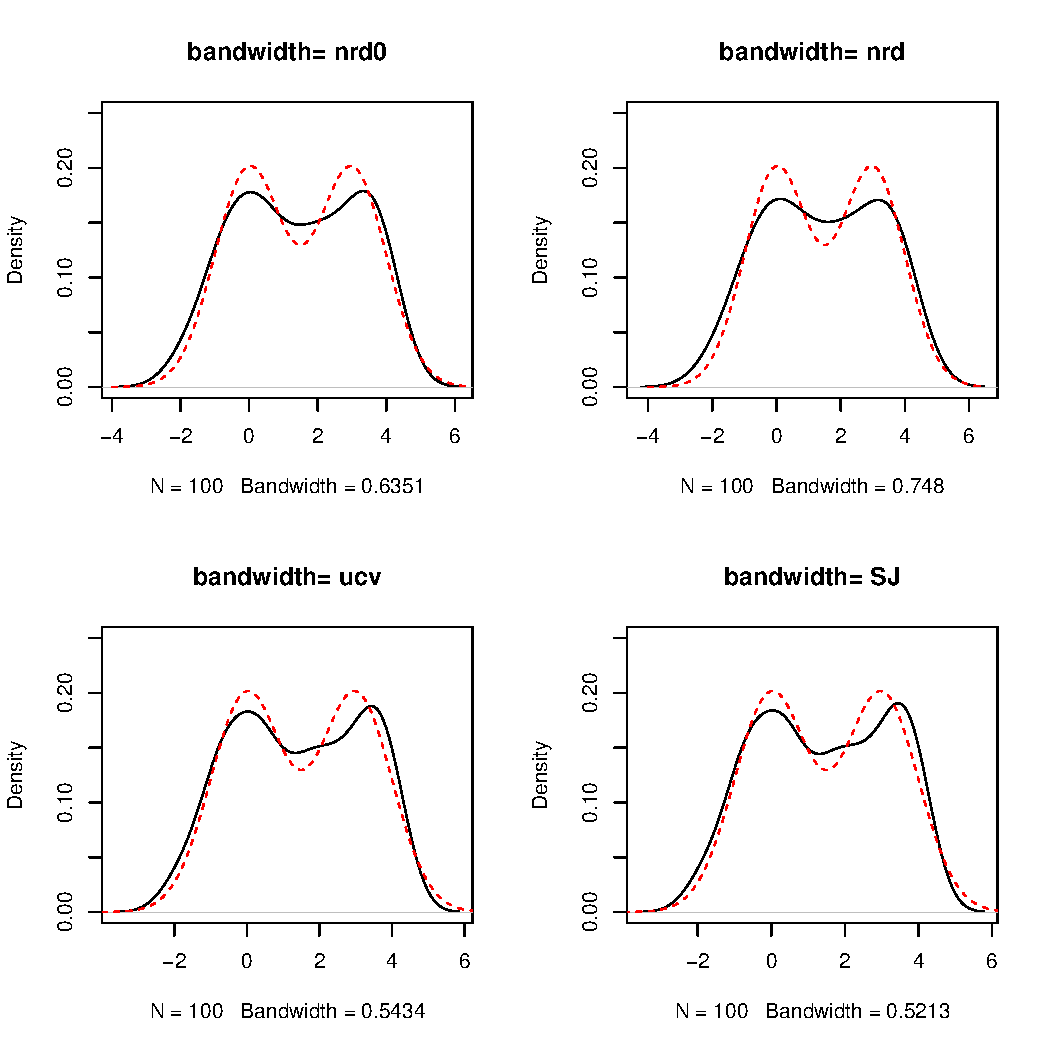
\includegraphics[width=\maxwidth]{figure/ten9} 
\begin{kframe}\begin{alltt}
\hlkwd{par}(mfrow = \hlkwd{c}(1, 1))
\end{alltt}
\end{kframe}
\end{knitrout}

The ``ucv" bandwidth appears to have picked up the two modes well but it also picked up some of the noise.  The ``nrd0" appears to have the best approximation of the density without the noise.\\

\item[10.a]  Bivariate kernel density estimate.\\

\begin{knitrout}
\definecolor{shadecolor}{rgb}{0.969, 0.969, 0.969}\color{fgcolor}\begin{kframe}
\begin{alltt}
dat <- \hlkwd{read.csv}(\hlstr{"C:/Users/dominic/Documents/StatsGIDP/Statistics papers and courses/STAT675-StatisticalComputing/ToraasonA2.csv"})
d.est <- \hlkwd{kde2d}(dat$x, dat$y)
\hlkwd{contour}(d.est)
\end{alltt}
\end{kframe}
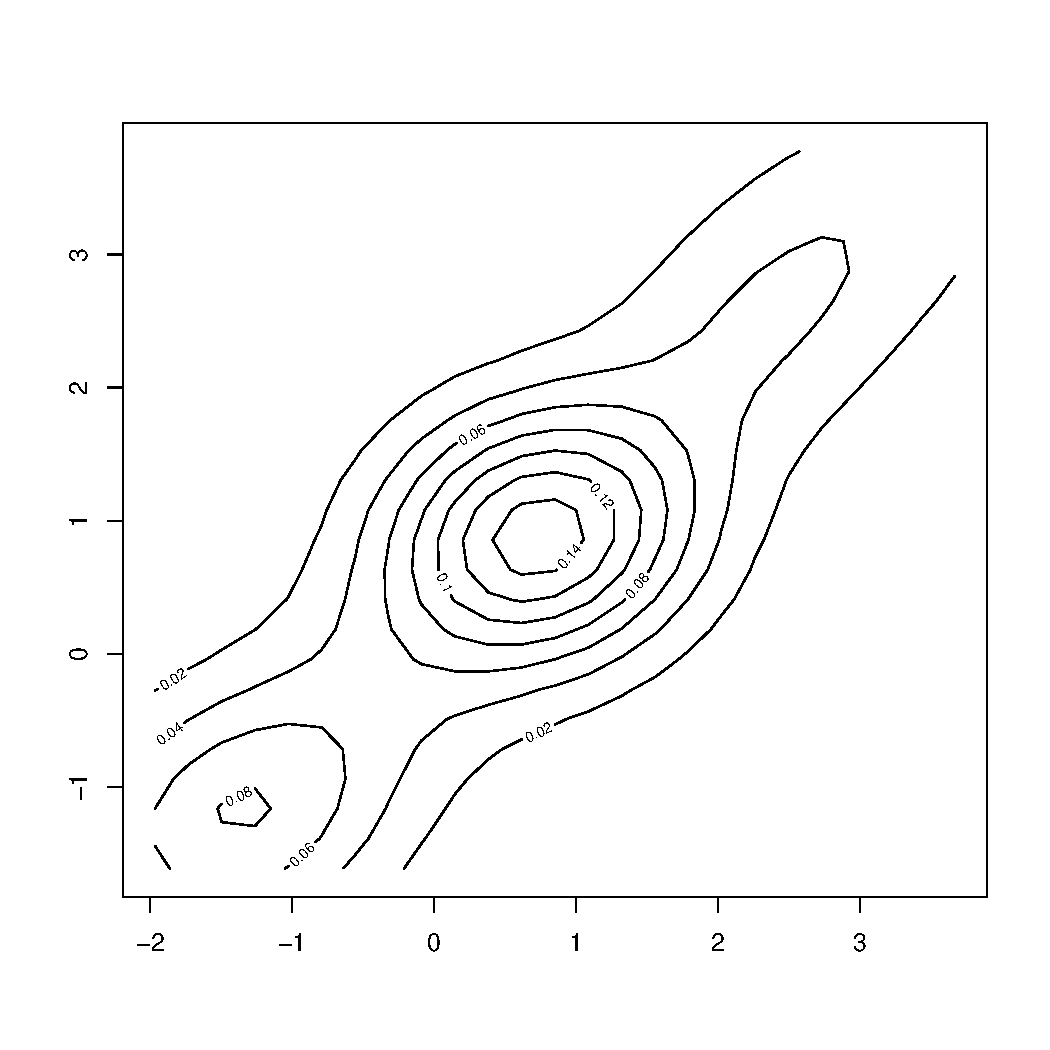
\includegraphics[width=\maxwidth]{figure/tena1} 
\begin{kframe}\begin{alltt}

\hlkwd{persp}(d.est, phi = 30, theta = 75, d = 5, col = \hlstr{"blue"}, shade = 0.25)
\end{alltt}
\end{kframe}
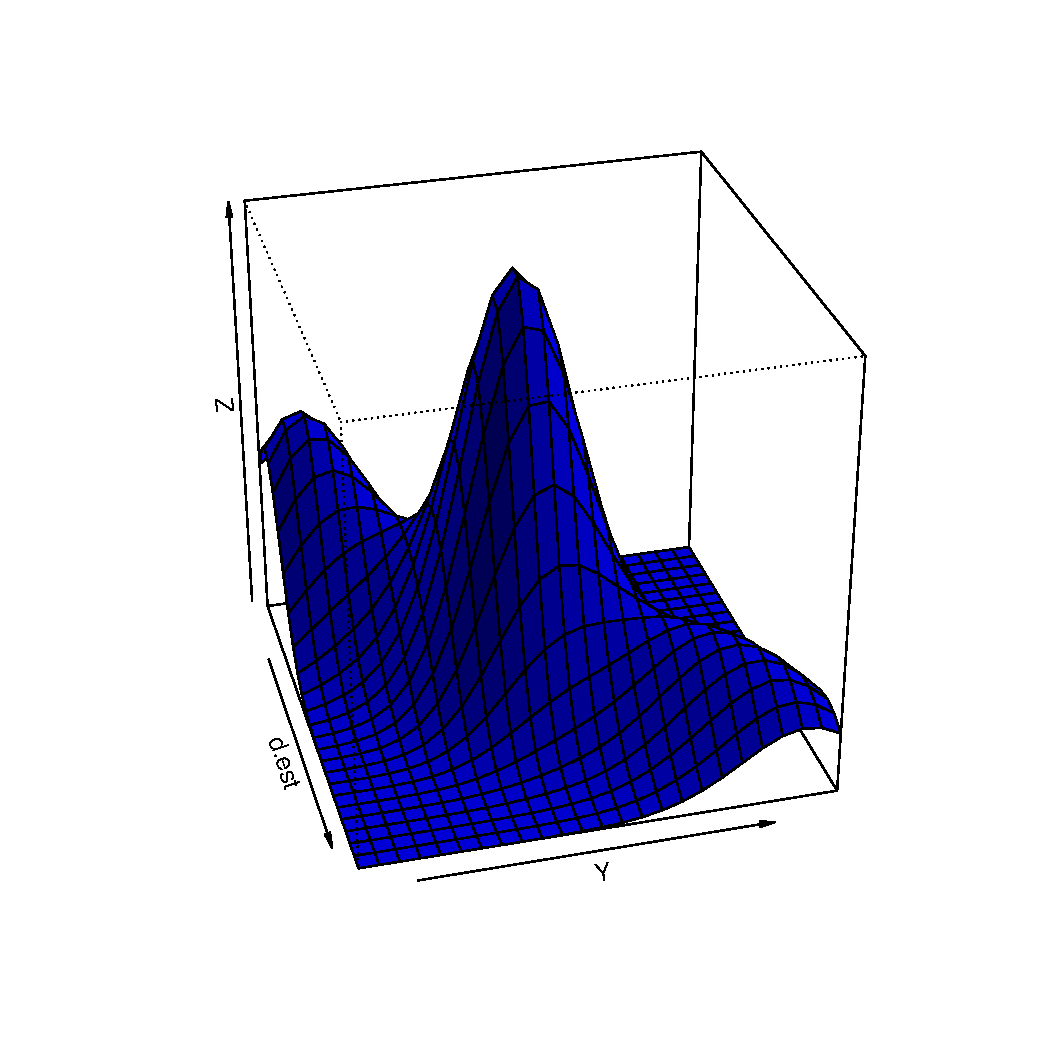
\includegraphics[width=\maxwidth]{figure/tena2} 

\end{knitrout}

\end{itemize}
\end{document}
